\documentclass[t]{beamer}
%\documentclass[handout]{beamer}
\usepackage[T1]{fontenc} % korrekte Trennung bei Wörtern mit Umlauten
\usepackage{ucs}\usepackage[utf8x]{inputenc} % allow äöü in text

% psnup -2 -r x.ps x2.ps

\usepackage{natbib}

\usetheme{Warsaw}
\useoutertheme{splitinfo} % self-made
%\useoutertheme[compressed]{miniframes}
%\setbeamercovered{transparent}
%\usecolortheme{albatross}
\usecolortheme{whale}

\title[Modelling atmospheric chemistry with CAABA/MECCA]{Modelling
  atmospheric chemistry with the CAABA/MECCA box model}

\author[Rolf Sander] {Rolf Sander}

\institute{Max-Planck Institute for Chemistry, Mainz, Germany}

\date{CAABA/MECCA workshop\\
Mainz} % , YEAR

% If you wish to uncover everything in a step-wise fashion, uncomment
% the following command:
% \beamerdefaultoverlayspecification{<+-| alert@+>}

% define \chem{} to print chemical formula
\DeclareRobustCommand*{\chem}[1]{\ensuremath{%
\mathcode`-="0200\mathcode`\=="003D% no space around "-" and "="
\mathrm{#1}}}

% define \unit{} to print a physical unit
\DeclareRobustCommand*{\unit}[1]{\ensuremath{%
\def\mu{\mbox{\textmu}}\def~{\,}%
\mathrm{#1}}}

\newcommand{\todo}[1]{{\uppercase{\bf ((TODO: #1))}}}
\newcommand{\E}[1]{\mbox{}\ensuremath{\times 10^{#1}}}
\def\TO{\mbox{}\ensuremath{\rightarrow}}
\def\TOHap{\mbox{}\ensuremath{\stackrel{\fac{Hap}}{\rightarrow}}}
\def\TOHV{\mbox{}\ensuremath{\stackrel{h\nu}{\rightarrow}}}
\def\EQ{\mbox{}\ensuremath{\rightleftharpoons}}

\begin{document}

%%%%%%%%%%%%%%%%%%%%%%%%%%%%%%%%%%%%%%%%%%%%%%%%%%%%%%%%%%%%%%%%%%%%%%%%%%%%%%

\begin{frame}%[shrink]
  \titlepage
\end{frame}

%%%%%%%%%%%%%%%%%%%%%%%%%%%%%%%%%%%%%%%%%%%%%%%%%%%%%%%%%%%%%%%%%%%%%%%%%%%%%%

\section{Agenda}

\begin{frame}

  \frametitle{Agenda}

  \begin{itemize}
  \item \textcolor{red}{PART I: THEORY}
    \begin{itemize}
    \item General Introduction to CAABA/MECCA
    \item Running CAABA/MECCA: A demonstration
    \end{itemize}
  \item \textcolor{red}{BREAK}
  \item \textcolor{red}{PART II: PRACTICE}
    \begin{itemize}
    \item The virtual machine
    \item Running the model
    \item Plotting the results
    \item Performing sensitivity studies
    \item Adapting the model to your project
    \end{itemize}
  \end{itemize}
  
\end{frame}

%%%%%%%%%%%%%%%%%%%%%%%%%%%%%%%%%%%%%%%%%%%%%%%%%%%%%%%%%%%%%%%%%%%%%%%%%%%%%%

% \section*{Table of Contents}

% \begin{frame}
%   \tableofcontents
% \end{frame}

%%%%%%%%%%%%%%%%%%%%%%%%%%%%%%%%%%%%%%%%%%%%%%%%%%%%%%%%%%%%%%%%%%%%%%%%%%%%%%

\section{Introduction}

\begin{frame}

  \frametitle{Introduction}

  \begin{itemize}
  \item Many atmospheric chemistry models have been developed in the
    past decades.
  \item Models vary strongly in complexity and efficiency.
  \item Each aimed at a particular goal, e.g.\ tropospheric or
    stratospheric chemistry\dots
  \item Often no clear separation between meteorological and chemical
    part of the model.
  \item When merging different chemistry mechanisms, often
    incompatibilities between codes occur.
  \item MESSy contains the comprehensive and flexible atmospheric
    chemistry module
    \begin{center}
      {\large\bf MECCA}\\
      (\underline{M}odule \underline{E}fficiently
      \underline{C}alculating the \underline{C}hemistry of the
      \underline{A}tmosphere).
    \end{center}
  \end{itemize}

\end{frame}

%%%%%%%%%%%%%%%%%%%%%%%%%%%%%%%%%%%%%%%%%%%%%%%%%%%%%%%%%%%%%%%%%%%%%%%%%%%%%%

\section{CAABA/MECCA Model Description}
\subsection{MECCA Chemistry}

\begin{frame}

  \frametitle{MECCA Chemistry}

  \begin{itemize}
  \item 699 gas phase species:
    \begin{itemize}
    \item 1789 reactions
    \item 384 photolysis reactions
    \end{itemize}
  \item 89 aqueous phase species:
    \begin{itemize}
    \item 145 reactions
    \item 47 gas-aqueous mass transfer reactions
    \item 34 acid/base and other equilibria
    \end{itemize}
  \item Basic \chem{O_3}, \chem{CH_4}, \chem{HO_x}, and \chem{NO_x}
    chemistry
  \item Tropospheric halogen (\chem{Cl}, \chem{Br}, \chem{I}) and sulfur
    (\chem{S}) chemistry from \citet{271} and \citet{1456}
  \item Tropospheric non-methane hydrocarbon (NMHC) chemistry and MOM
    isoprene/terpene mechanism \citep{2272}
  \item Stratospheric chemistry based on the model of \citet{1402} and
    the Mainz Chemical Box Model \citep{1608}
  \item Rate coefficients updated according to recent JPL and IUPAC
    recommendations
  \end{itemize}

\end{frame}

%%%%%%%%%%%%%%%%%%%%%%%%%%%%%%%%%%%%%%%%%%%%%%%%%%%%%%%%%%%%%%%%%%%%%%%%%%%%%%

%fragile allows to use verbatim in the frame
\begin{frame}[fragile]

  \frametitle{MECCA Chemistry}

  % the \beamerdefaultoverlayspecification{<+-| alert@+>}
  % does not seem to work in a fragile frame, so it must be added
  % explicitly to the itemize command here
  \begin{itemize}[<+-| alert@+>]
  \item Only one master file (\verb|gas.eqn|) for all gas-phase
    reactions, e.g.:\\
    \verb|<G1000> O2 + O1D = O3P + O2 : {%UpStTrG}|\\
    \verb|3.3E-11{|\textsection\verb|1.1}*EXP(55./temp); {&3245}|
  \item Reaction number: $<$G1000$>$
  \item Reaction string: \chem{O_2} + \chem{O(^1D)} \TO\ \chem{O(^3P)} +
    \chem{O_2}
  \item User-selected subset \verb|{%UpStTrG}| using reaction labels:
    \begin{itemize}[<*>]
    \item \verb|Up| = upper atmosphere
    \item \verb|St| = stratospheric reaction
    \item \verb|Tr| = tropospheric reaction
    \item \verb|G| = gas-phase reaction
    \end{itemize}
  \item Rate coefficient: $3.3\E{-11} \exp(55 \unit{K}/T)$ \unit{cm^3/s}
  \item Uncertainty factor for Monte-Carlo studies: 1.1 (about $\pm$ 10 \%)
  \item Reference information: 3245 = JPL recommendation (2015)
  \end{itemize}

\end{frame}

%%%%%%%%%%%%%%%%%%%%%%%%%%%%%%%%%%%%%%%%%%%%%%%%%%%%%%%%%%%%%%%%%%%%%%%%%%%%%%

\subsection{CAABA/MECCA Modularity}

\begin{frame}

  \frametitle{CAABA/MECCA Modularity}

  \begin{itemize}
  \item Very modular structure (MESSy standard by \citet{1664})
  \item Link to different meteorological base models\\
    \includegraphics[width=0.7\textwidth]{modular-mecca}
  \item CAABA = Chemistry As A Boxmodel Application
  \item Extensive testing in a box model
  \item Develop parameterization
  \item Run parameterization in global model runs
  \end{itemize}

\end{frame}

%%%%%%%%%%%%%%%%%%%%%%%%%%%%%%%%%%%%%%%%%%%%%%%%%%%%%%%%%%%%%%%%%%%%%%%%%%%%%%

\subsection{The CAABA box model}

\begin{frame}

  \frametitle{The CAABA Box Model}

  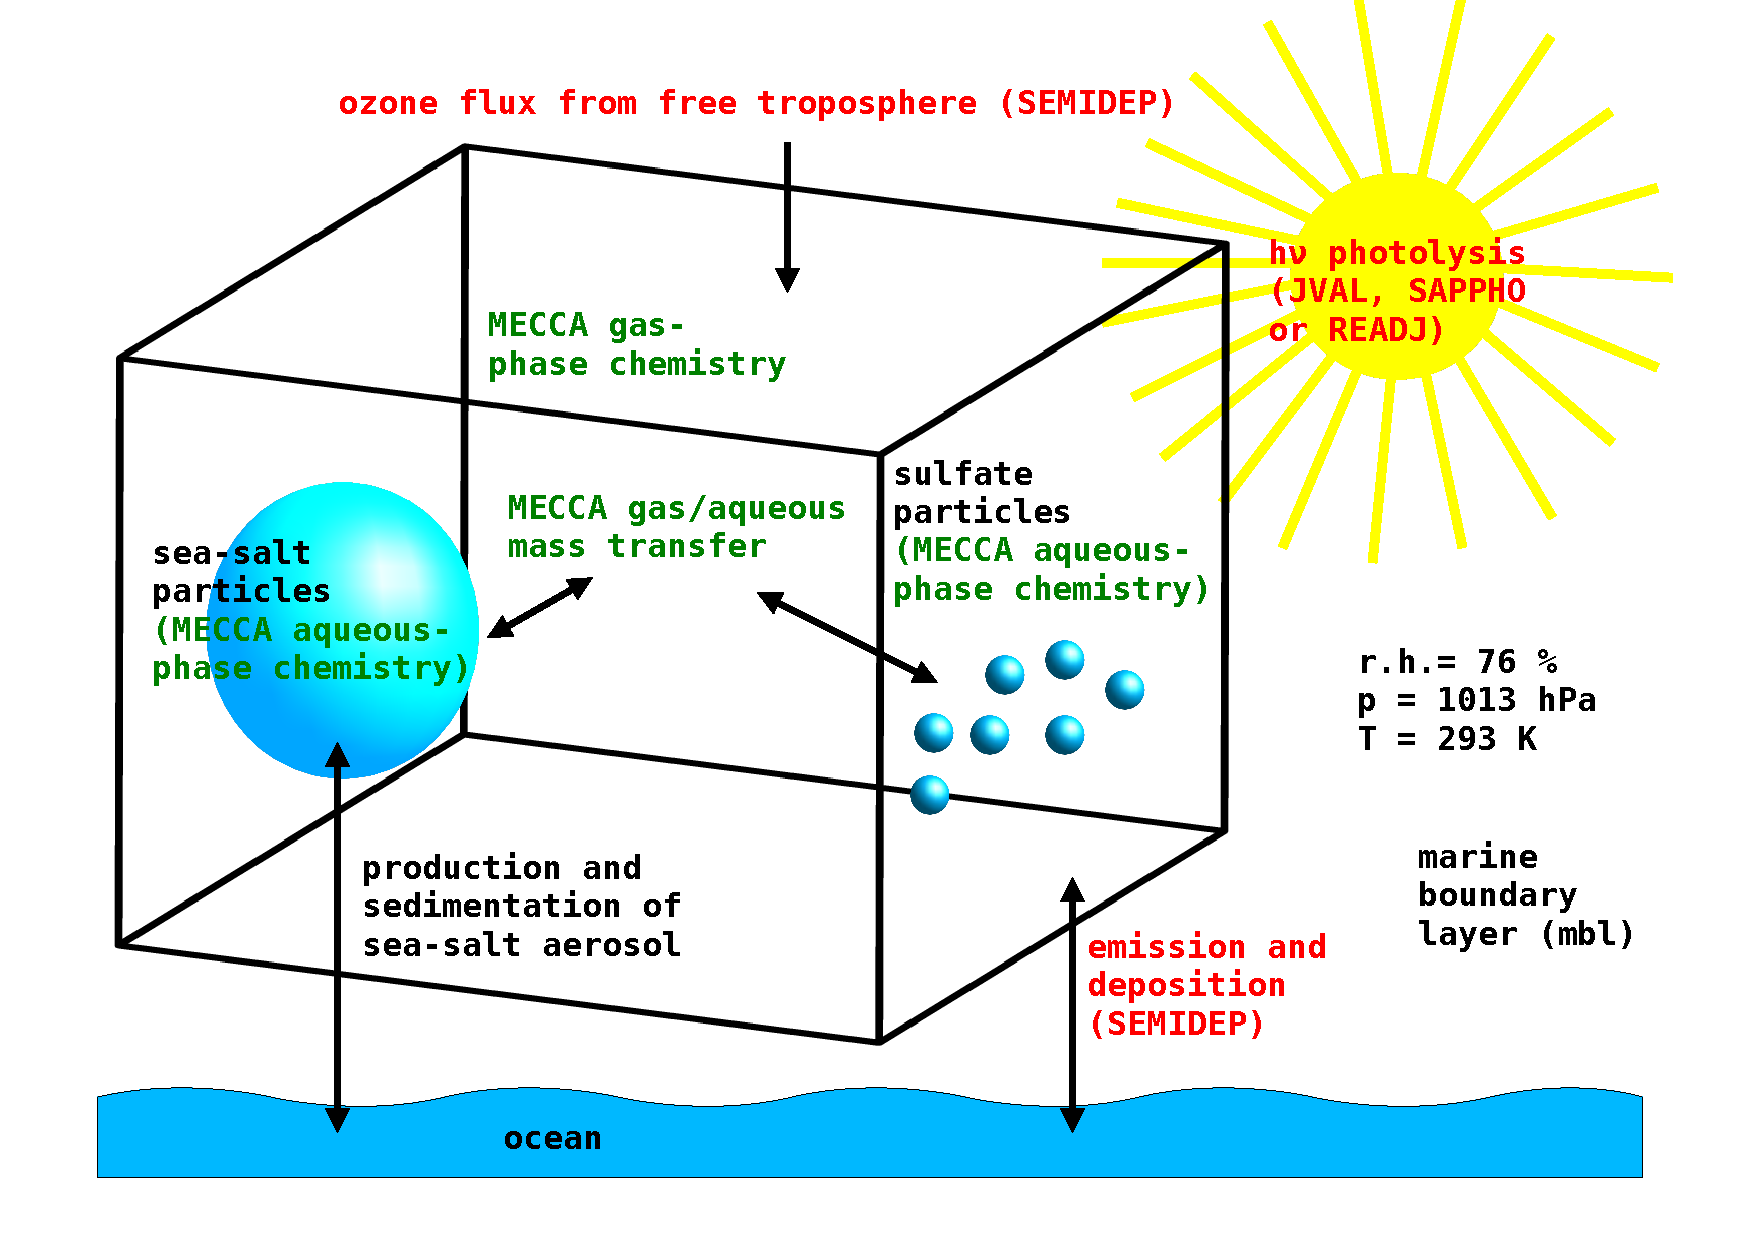
\includegraphics[width=0.9\textwidth]{caaba_sketch}

\end{frame}

%%%%%%%%%%%%%%%%%%%%%%%%%%%%%%%%%%%%%%%%%%%%%%%%%%%%%%%%%%%%%%%%%%%%%%%%%%%%%%

\subsection{The CAABA box model}

\begin{frame}

  \frametitle{Box Model Modes}
  \def\nosep{\setlength\parsep{0mm}\setlength\topsep{0mm}\setlength\itemsep{0mm}}

  \parbox[b]{0.6\textwidth}{{\bf Box mode:}\footnotesize
    \begin{itemize}\nosep
    \item static: constant $T$, $p$, rh
    \item dynamic: Lagrangian along trajectory, variable $T$, $p$, rh
    \end{itemize}}
  \fbox{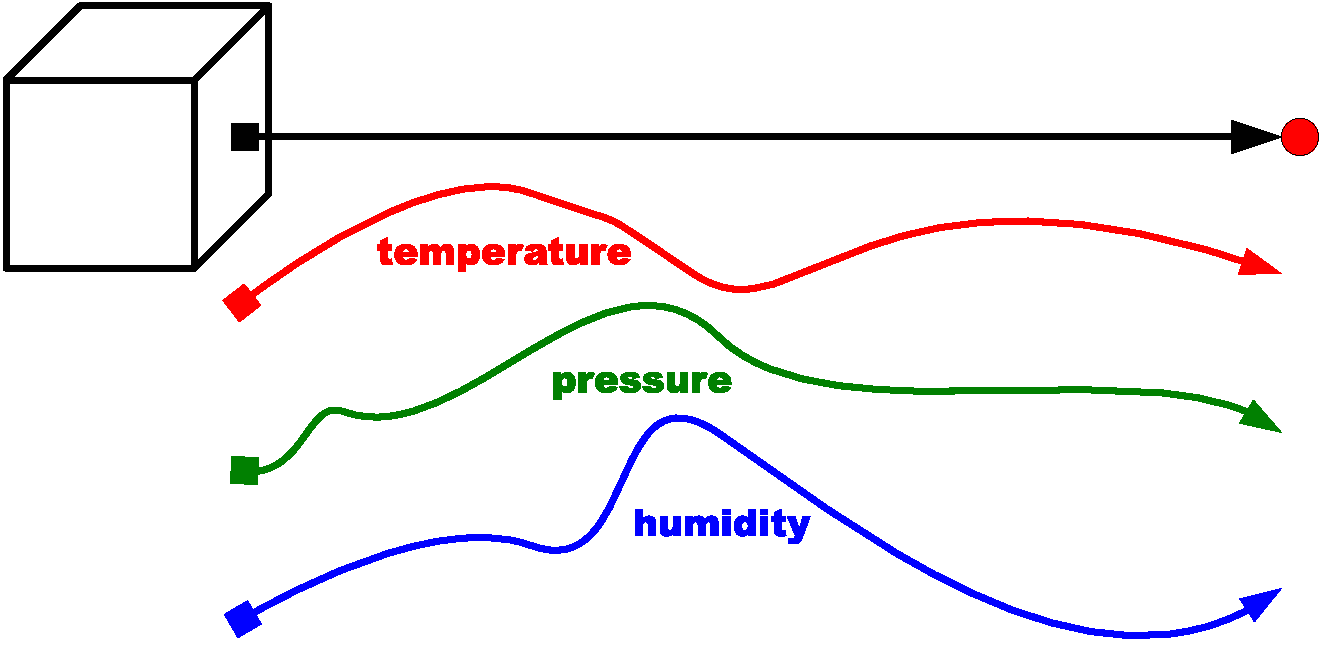
\includegraphics[width=0.3\textwidth]{box_model}}\\
  \parbox[b]{0.6\textwidth}{{\bf Steady-state mode:}\footnotesize
    \begin{itemize}\nosep
    \item initialize with measured long-lived species
    \item let short-lived species (e.g., OH, HO$_2$) run into steady
      state conditions
    \item multirun: one run for each measured data point
    \end{itemize}}
  \fbox{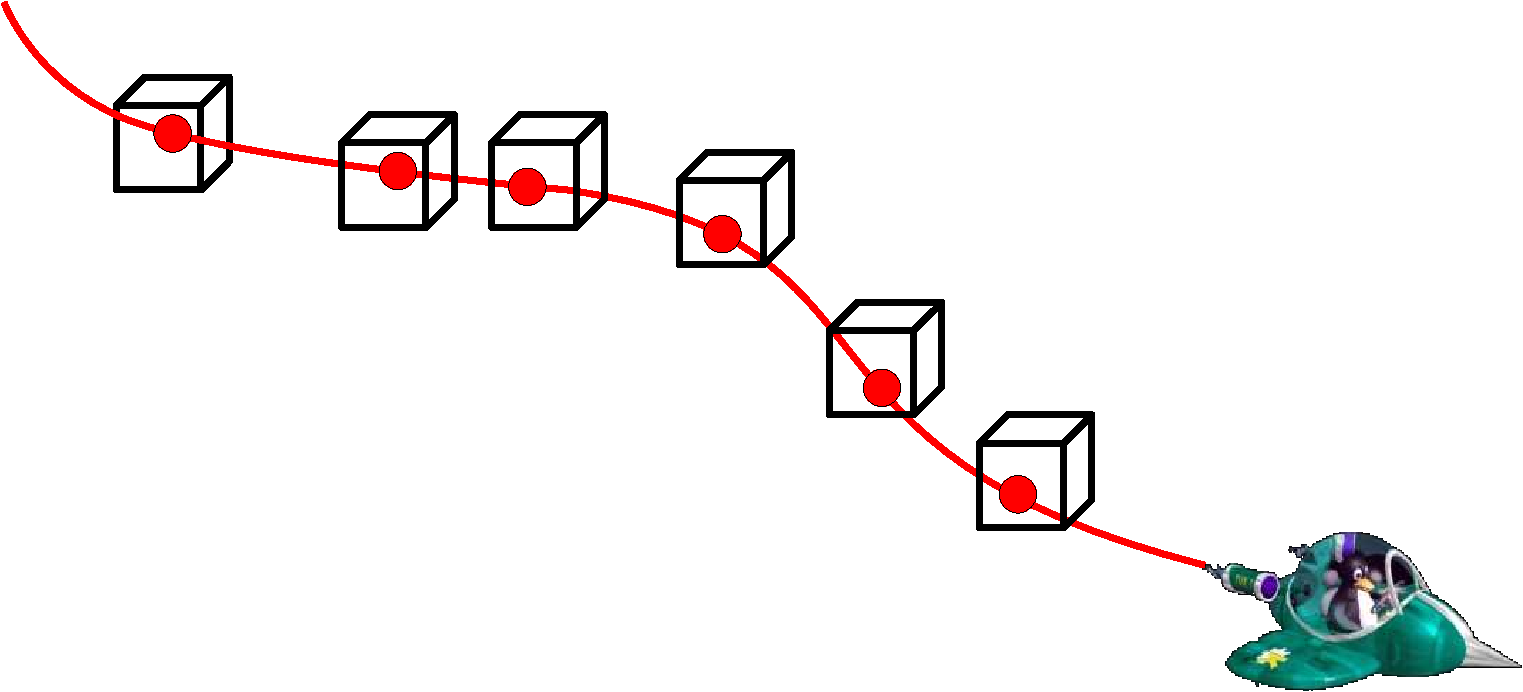
\includegraphics[width=0.3\textwidth]{steady_state_model}}\\
  \parbox[b]{0.6\textwidth}{{\bf Trajectory mode:}{\footnotesize
    \begin{itemize}\nosep
    \item initialize with data from global model
    \item model runs along trajectory
    \item multirun: one run for each measured data point
    \end{itemize}}
  {\bf Monte-Carlo mode:}\footnotesize
    \begin{itemize}\nosep
    \item variation of rate coefficients
    \end{itemize}}
  \fbox{\includegraphics[width=0.3\textwidth]{traject_model}}
  
\end{frame}

%%%%%%%%%%%%%%%%%%%%%%%%%%%%%%%%%%%%%%%%%%%%%%%%%%%%%%%%%%%%%%%%%%%%%%%%%%%%%%

\subsection{Namelists}

\begin{frame}

  \frametitle{Namelists}

  \begin{itemize}
  \item Control the behaviour of a CAABA/MECCA model run:
    \begin{itemize}
    \item temperature, pressure, humidity
    \item model start and duration
    \item output interval
    \item select submodels (MECCA, JVAL, SEMIDEP, TRAJECT, \dots)
    \item scenarios
    \item steady-state stop?
    \item trajectory file?
    \end{itemize}
  \item Default: use the same namelist as last time
  \item For testing: caaba\_simple.nml
  \end{itemize}

\end{frame}

%%%%%%%%%%%%%%%%%%%%%%%%%%%%%%%%%%%%%%%%%%%%%%%%%%%%%%%%%%%%%%%%%%%%%%%%%%%%%%

\subsection{Scenarios}

\begin{frame}

  \frametitle{Scenarios}

  \begin{itemize}
  \item describe boundary conditions:
    \begin{itemize}
    \item photolysis
    \item initialization
    \item emission
    \item dry deposition
    \end{itemize}
  \item available scenarios:
    \begin{itemize}
    \item {\bf MBL, OOMPH:} MBL chemistry
    \item {\bf FF\_ANTARCTIC, FF\_ARCTIC:} frost flowers and polar ODEs
    \item {\bf FREE\_TROP, HOOVER:} free troposphere
    \item {\bf STRATO, MTCHEM:} stratosphere and above
    \item {\bf LAB, LAB\_C15:} laboratory conditions (reaction chamber)
    \item {\bf MIM2:} for isoprene chemistry \citep{2272}
    \item {\bf ???:} add your own\dots
    \end{itemize}
  \item select your scenario in namelist file
  \end{itemize}

\end{frame}

%%%%%%%%%%%%%%%%%%%%%%%%%%%%%%%%%%%%%%%%%%%%%%%%%%%%%%%%%%%%%%%%%%%%%%%%%%%%%%

\subsection{Further Information}

\begin{frame}

  \frametitle{Further Information}

  \begin{itemize}%[<+-| alert@+>]
  %\item Collaboration encouraged, let's work together!
  \item Web page:\\
    \url{http://www.mecca.messy-interface.org}
  \item CAABA/MECCA model description paper:\\
    Sander et al. (2011), GMD, 4, 373-380\\
    \url{http://www.geosci-model-dev.net/4/373}
  \item User manual:\\
    manual/caaba\_mecca\_manual.pdf
  \item GPL License
  %\item Acknowledgements or co-authorship?
  % \item Make code additions available (which can eventually be
  %   incorporated into main CAABA/MECCA code)
  \end{itemize}

\end{frame}

%%%%%%%%%%%%%%%%%%%%%%%%%%%%%%%%%%%%%%%%%%%%%%%%%%%%%%%%%%%%%%%%%%%%%%%%%%%%%%

\subsection{Demo}

\begin{frame}

  \vfill
  \begin{center}
    {\Large\bf NEXT:\\[1cm]
    On-screen demo of model run}
  \end{center}
  \vfill

\end{frame}

%%%%%%%%%%%%%%%%%%%%%%%%%%%%%%%%%%%%%%%%%%%%%%%%%%%%%%%%%%%%%%%%%%%%%%%%%%%%%%

\section*{Bibliography}

% for unknown reasons, newblock is currently undefined:
\def\newblock{}
% reset overlay to avoid that all references are shown one after another:
\beamerdefaultoverlayspecification{}

\begin{frame}[shrink]
\bibliographystyle{egu}    % bst file
\bibliography{literat,www} % bib files

\end{frame}

%%%%%%%%%%%%%%%%%%%%%%%%%%%%%%%%%%%%%%%%%%%%%%%%%%%%%%%%%%%%%%%%%%%%%%%%%%%%%%

\end{document}
